\documentclass{article}
\usepackage[pdftex]{graphicx}
\usepackage{amsmath}
\usepackage{verbatim}
\author{Michael Anderson}
\title{Homework Set 3}
\begin{document}
\maketitle
\center{CS533}
\center{Prof. Fern}\\
\flushleft
\newpage

\begin{enumerate}
\item[\textbf{1.}]
Consider the following MDP:

$S = \{s_1, s_2, s_3, s_4\}$\\
$A = \{a_1, a_2\}$\\
$R = \{(s_1, 0), (s_2, 1), (s_3, 3), (s_4, 2)\}$\\
$T = \{(s_1,a_1,s_2,1), (s_1,a_2,s_4,1) (s_2,a_1,s_3,1), (s_2,a_2,s_3,1),$\\
$(s_3,a_1,s_3,1), (s_3,a_2,s_3,1), (s_4,a_1,s_4,1), (s_4,a_2,s_4,1)\}$

This MDP looks like:

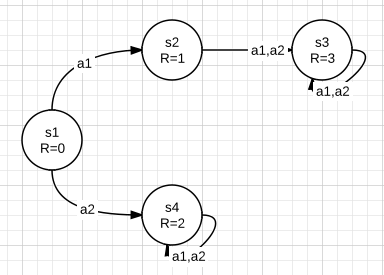
\includegraphics{mdp1.png}

For the optimal stationary policy, if an agent starts at $s_1$, then it should
clearly take $a_1$. In that way once the agent moves to $s_2$, and then further to $s_3$, they will end up trapped in a state with a lot of reward.

For the optimal non-stationary policy, suppose that the finite horizon $h$ is
only one. Now if the agent is at $s_1$, it should clearly take $a_2$, to grab
the largest reward reachable in one action, which is at $s_4$.

\item[\textbf{2.}]
\begin{enumerate}
\item[a)]
Let the STRIPS problem be called $S$, and the MDP be called $M$.

There will be a state in $M$ for each true/false combinations of the
propositions in $S$. E.g., if $S$ has two propositions $p_1$ and $p_2$, then
$M$ has the four
states $\{p_1p_2, p_1 \neg p_2, \neg p_1p_2, \neg p_1 \neg p_2\}$.

Every single action in $S$ maps directly to a single action in $M$.

States in $M$ that have each of the propositions in the goal of $S$ will have
a reward of 1. All other states have a reward of 0.

The transition function of $M$ is determined by the PRE, ADD, and DEL effects
of each action in $S$. Iff a state $s$ in $M$ has the preconditions necessary
for some action $a$, there will be some entry $(s,a,s')$ in the transition
function such that $s'$ is simply $s$ with all of the ADD effects of $a$ set
to true, and the DEL effects of $a$ set to false. Since STRIPS actions are
deterministic, $T(s,a,s') = 1$ for all such actions added in this way.

\item[b)]
Since the state space of $M$ is the enumeration of the possible true/false
combinations of propositions of $S$, there are $2^n$ states in $M$.

\item[c)]
Each of the $2^n$ states has a tree of width $m$ (the number of actions), and
of depth $h$, leading to a time complexity of $2^nmh$ using dynamic programming.

\end{enumerate}

\item[\textbf{3.}]
\begin{enumerate}
\item[a)]
Make the recurrence relation of the policy evaluation algorithm:

\[
V^k_\pi(s) = R(s) + \sum_{s' \, in \, NEXT(s,\pi(s,k))}
T(s,\pi(s,k),s')V^{k-1}_\pi(s')
\]

In other words, instead of considering all possible $s'$s that could result
from the action recommended by $\pi$, only consider $s'$s that are reachable
from (s,a) with non-zero probability. This reduces the time complexity of the
algorithm from $O(hmn^2)$ to $O(hmnr)$, which is strictly better if $r < n$.
\item[b)]
Make the recurrence relation of the value iteration algorithm:

\[
V^k(s) = R(s) + \max_{a \, in \, LEGAL(s)} \sum_{s' \, in \, NEXT(s,a))}
T(s,a,s')V^{k-1}
\]

In other words, only consider actions that are actually takeable from $s$, and
as in part a) only consider $s'$s that are reachable from (s,a) with non-zero
probability. This reduces the time complexity of the algorithm from $O(hmn^2)$
to $O(hknr)$, which is strictly better if $r < n$ and $k < m$.

\end{enumerate}
\end{enumerate}
\end{document}
